
%%%%%%%%%%%%%%%%%%%%%%%%%%%%%%%%%%%%%%%%%%%%%%%%%%%%%%%%%%%%%%%%%%%%%%%%%%%%%%%%%%%%%%%%%%%%%%%%%%%%%%%%%%%%%%%%%%%%%%%%%%%%%%%%%%%%%%%%%%%%%%%%%%%%%%%%%%%%%%%%%%%%
\chapter{How do I compare genomic data in Ondex?}
\label{cha:comp}
%%%%%%%%%%%%%%%%%%%%%%%%%%%%%%%%%%%%%%%%%%%%%%%%%%%%%%%%%%%%%%%%%%%%%%%%%%%%%%%%%%


\section*{Application case: Combining comparative genomics with data integration for the prediction of potential pathogenicity genes}
\label{sec:phi_bot_app}
We integrated PHI-base (\url{http://www.phi-base.org/}), a database containing expertly curated molecular and biological information on genes 
proven to affect the outcome of pathogen-host interactions. 
Additionally, we loaded the genome sequence of \textit{Botrytis cinerea} (\url{http://www.broad.mit.edu/annotation/genome/botrytis_cinerea/}).
See section \ref{sec:integrator} for more information.

Running our implementation of the InParanoid algorithm\footnote{Remm M., Storm C.E., Sonnhammer E.L. (2001). 
``Automatic clustering of orthologs and in-paralogs from pairwise species comparisons''. Journal of Molecular Biology, 314(5):1041-52, PubMed ID: 11743721.}
based on BLAST mappings of the genomic data gives us new biological insights. 
Indeed PHI-base contains a lot of annotation which can be displayed on the network using the ``Annotators'' menu. 
This type of visualization in Ondex allows us to gain new hypotheses on the \textit{Botrytis} genome.

After loading the data file botrytis\_phibase.oxl from the directory Tutorial\_files/Application\_cases, a metagraph is displayed. 
The metagraph (see Figure \ref{fig:bot_metagraph}) shows red circles are proteins from \textit{Botrytis} and blue triangles are proteins from PHI-base 
(see explanation for ``Interaction:Protein'' in section \ref{sec:integrator}).

\begin{figure}[H]
\centering
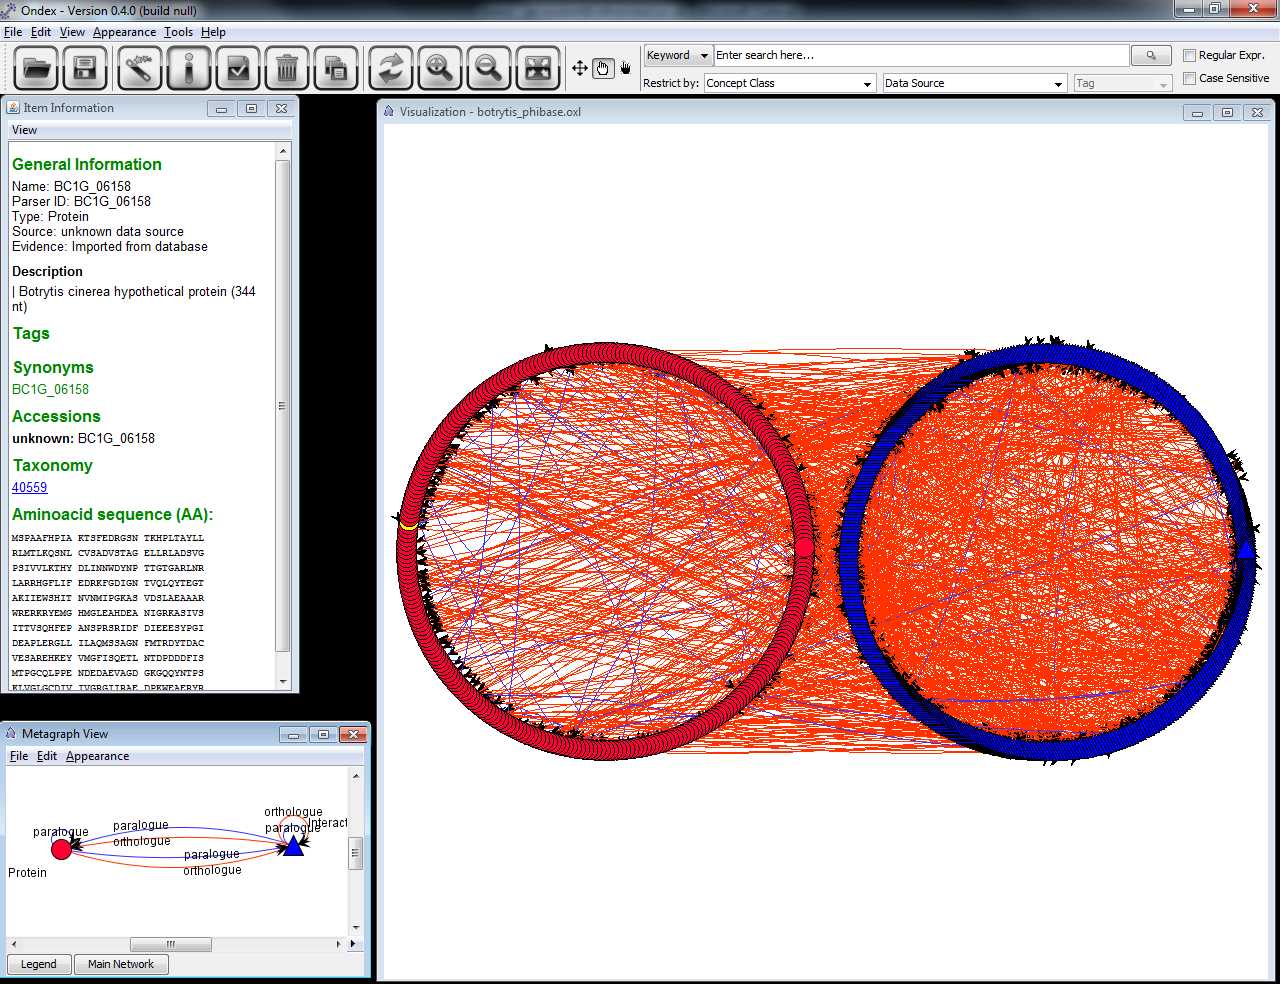
\includegraphics[scale=0.35]{images/Oct12/app2fig1.png} 
\caption{Circular layout, metagraph and item information window}
\label{fig:bot_metagraph}
\end{figure}

They are linked by orthologue and paralogue relations indicating whether genes were separated by the event of speciation (ortholog) or 
genetic duplication (paralog). 
Orthologs retain the same function in the course of evolution, whereas paralogs evolve new functions, even if these are related to the original one. 
Concepts imported from PHI-base contain a lot of annotation. 
In order to make this annotation visible, we are going to use the ``Annotators'' menu. 
First of all, let us use the ``Colour Concepts by General Attribute'' annotator (see Figure \ref{fig:bot_colbyval}).

\begin{figure}[H]
\centering
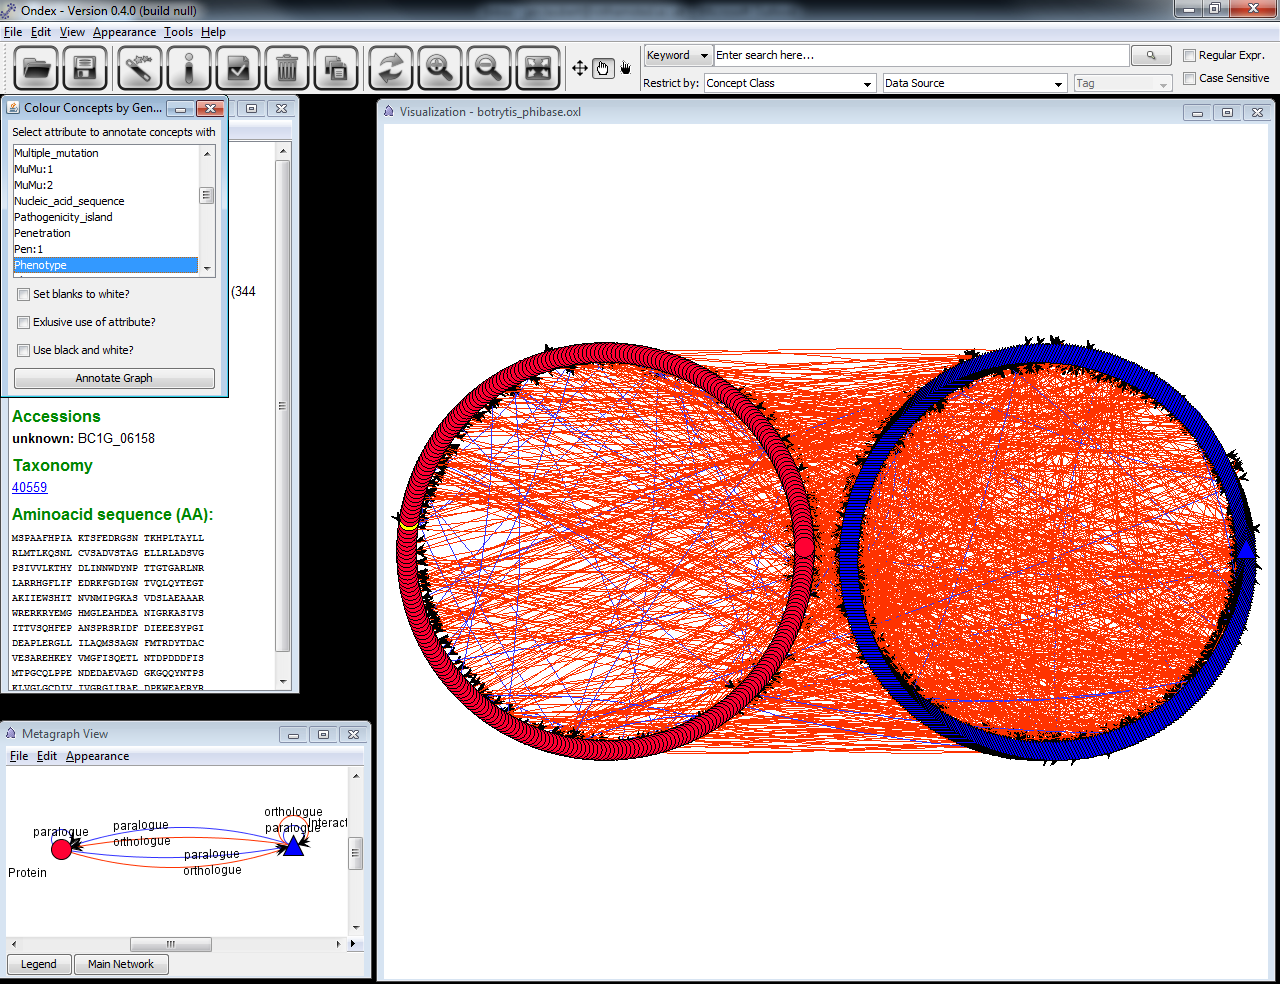
\includegraphics[scale=0.35]{images/Oct12/app2fig2.png} 
\caption{Colour Concepts by General Attribute annotator}
\label{fig:bot_colbyval}
\end{figure}

As a lot of phenotypic information is encoded in PHI-base, we select the first attribute: ``Phenotype''. 
Then click on ``Annotate Graph''. 
We get a colour legend and colour annotation on the triangles (PHI-base concepts) 
in the graph as shown in Figure \ref{fig:bot_colbyval_res}.

\begin{figure}[H]
\centering
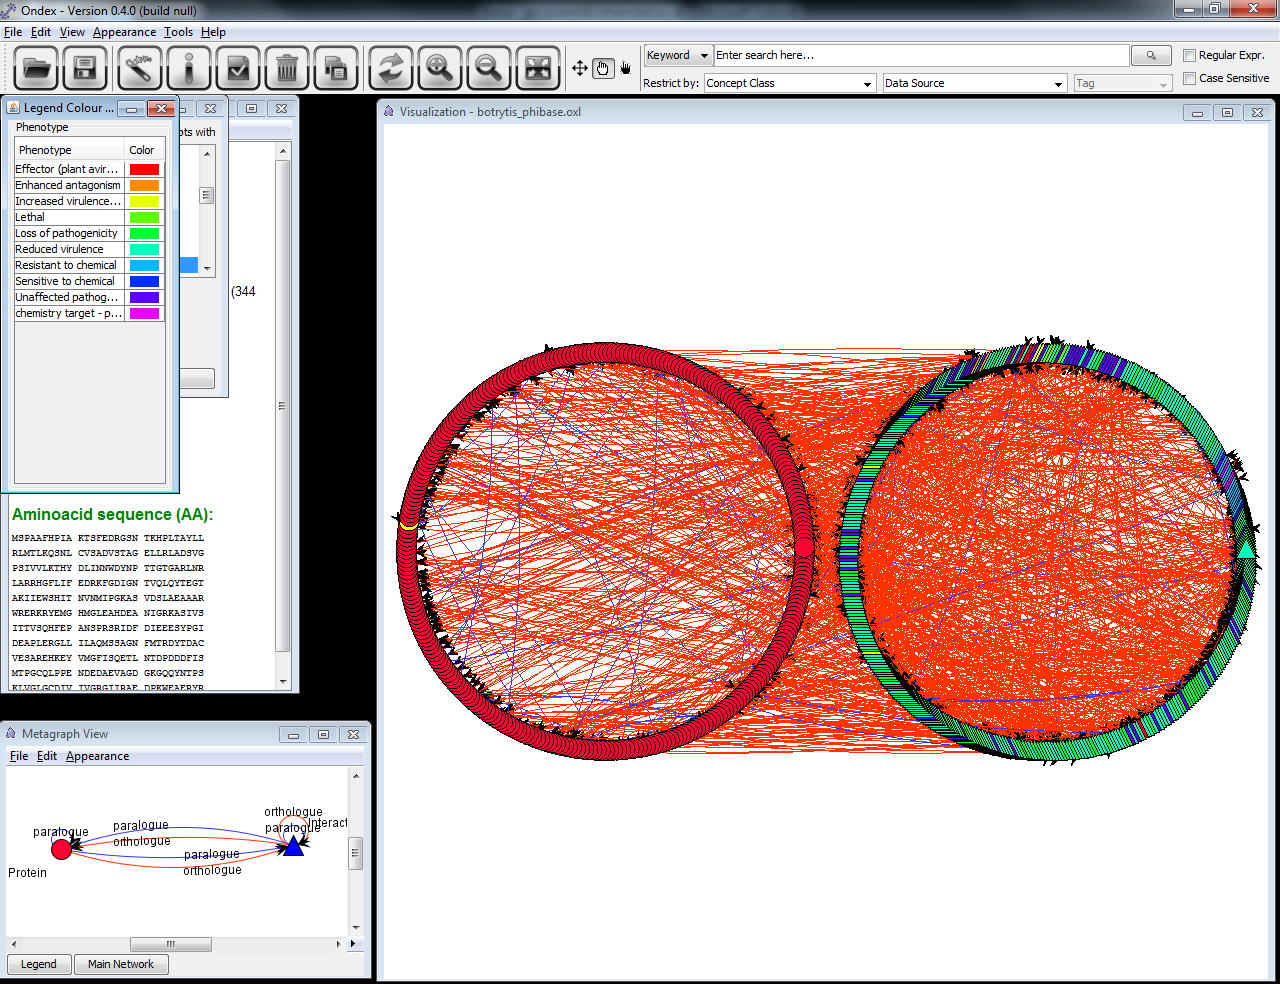
\includegraphics[scale=0.35]{images/Oct12/app2fig3.png} 
\caption{Results of the Colour Concepts by General Attribute annotator}
\label{fig:bot_colbyval_res}
\end{figure}

We use Appearance $->$ Layouts $->$ Gem in order to visualize clusters (see Figure \ref{fig:bot_gem}).

\begin{figure}[H]
\centering
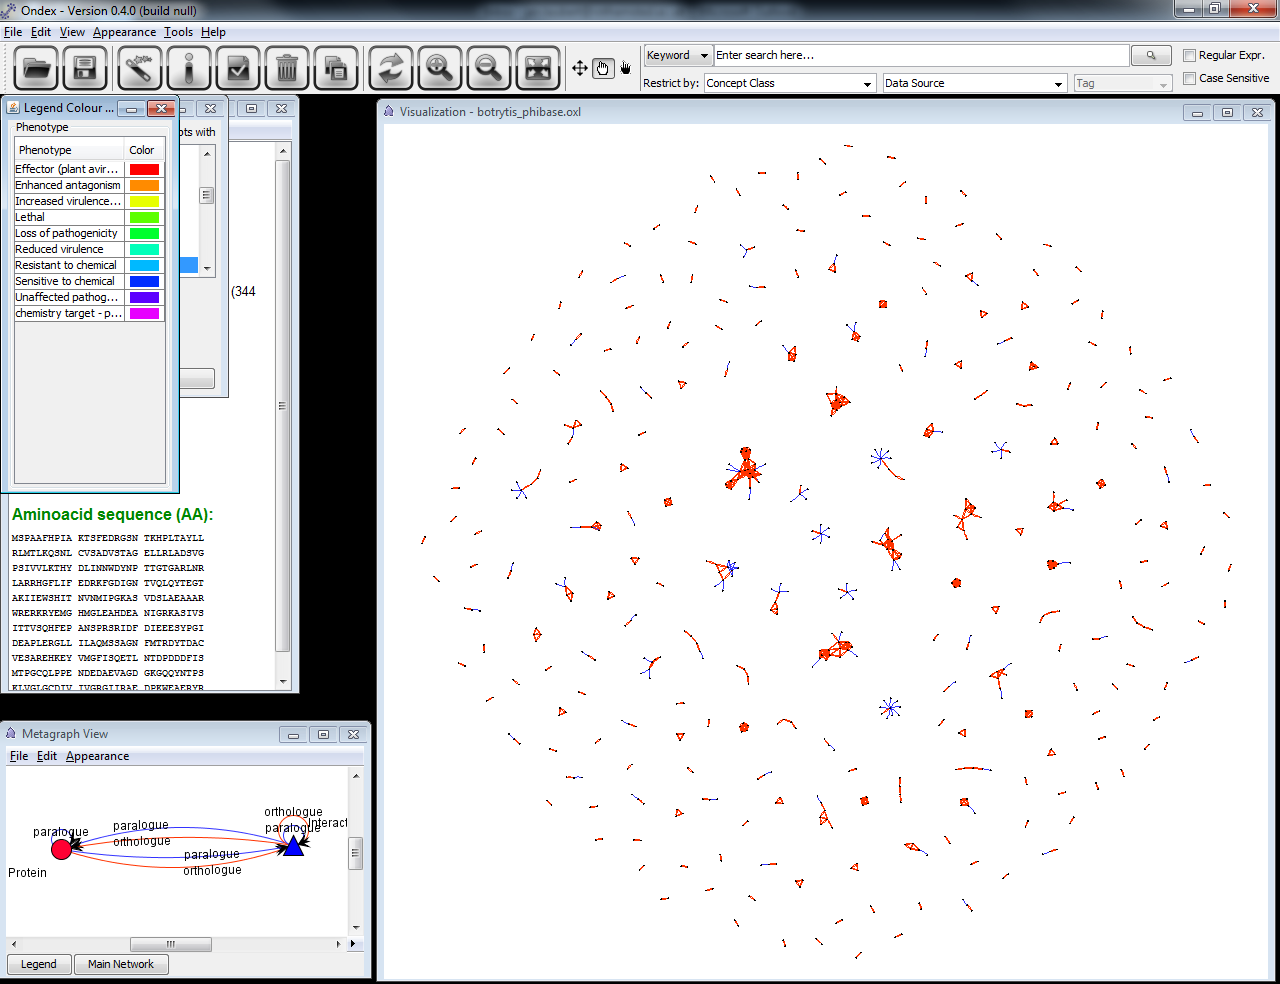
\includegraphics[scale=0.35]{images/Oct12/app2fig4.png} 
\caption{After applying the Gem layout}
\label{fig:bot_gem}
\end{figure}

We may now zoom in on a particular cluster as shown in Figure \ref{fig:bot_zoom_in}.

\begin{figure}[H]
\centering
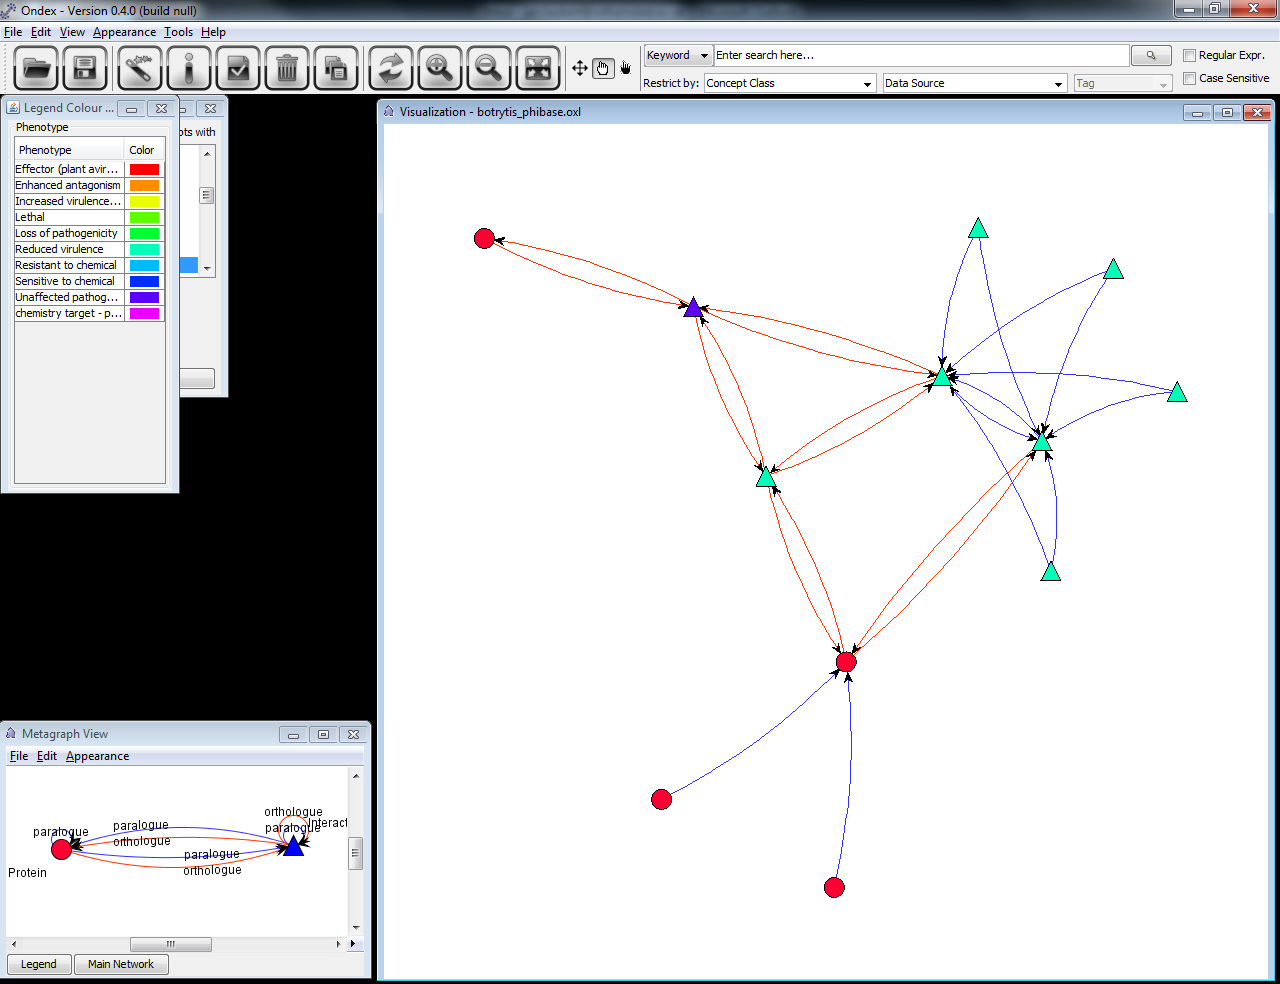
\includegraphics[scale=0.35]{images/Oct12/app2fig5.png} 
\caption{Zooming in on a cluster}
\label{fig:bot_zoom_in}
\end{figure}

Another Annotator we may use is the ``Shape Concepts by General Attribute'' annotator as PHI-base also contains information about the pathogen species. 
We select the attribute ``Taxonomy\_ID'' (NCBI Taxonomy Identifier) in the list as shown in Figure \ref{fig:bot_taxid}.

\begin{figure}[H]
\centering
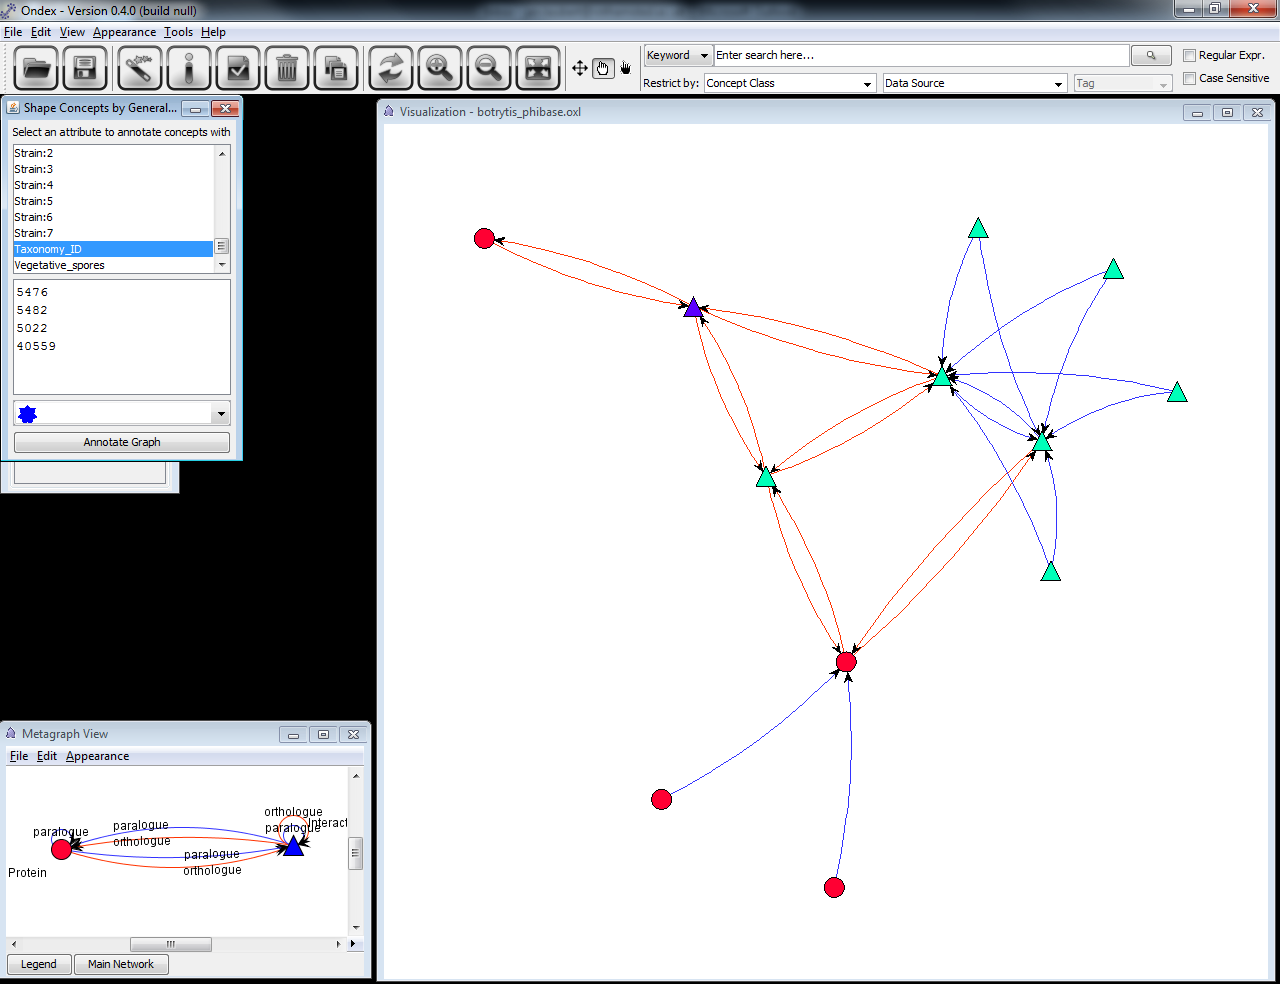
\includegraphics[scale=0.35]{images/Oct12/app2fig6.png} 
\caption{Selecting an attribute}
\label{fig:bot_taxid}
\end{figure}

We can look up the concepts' Taxonomy identifier in their corresponding Item Information as shown in Figure \ref{fig:bot_taxid_lookup1}.

\begin{figure}[H]
\centering
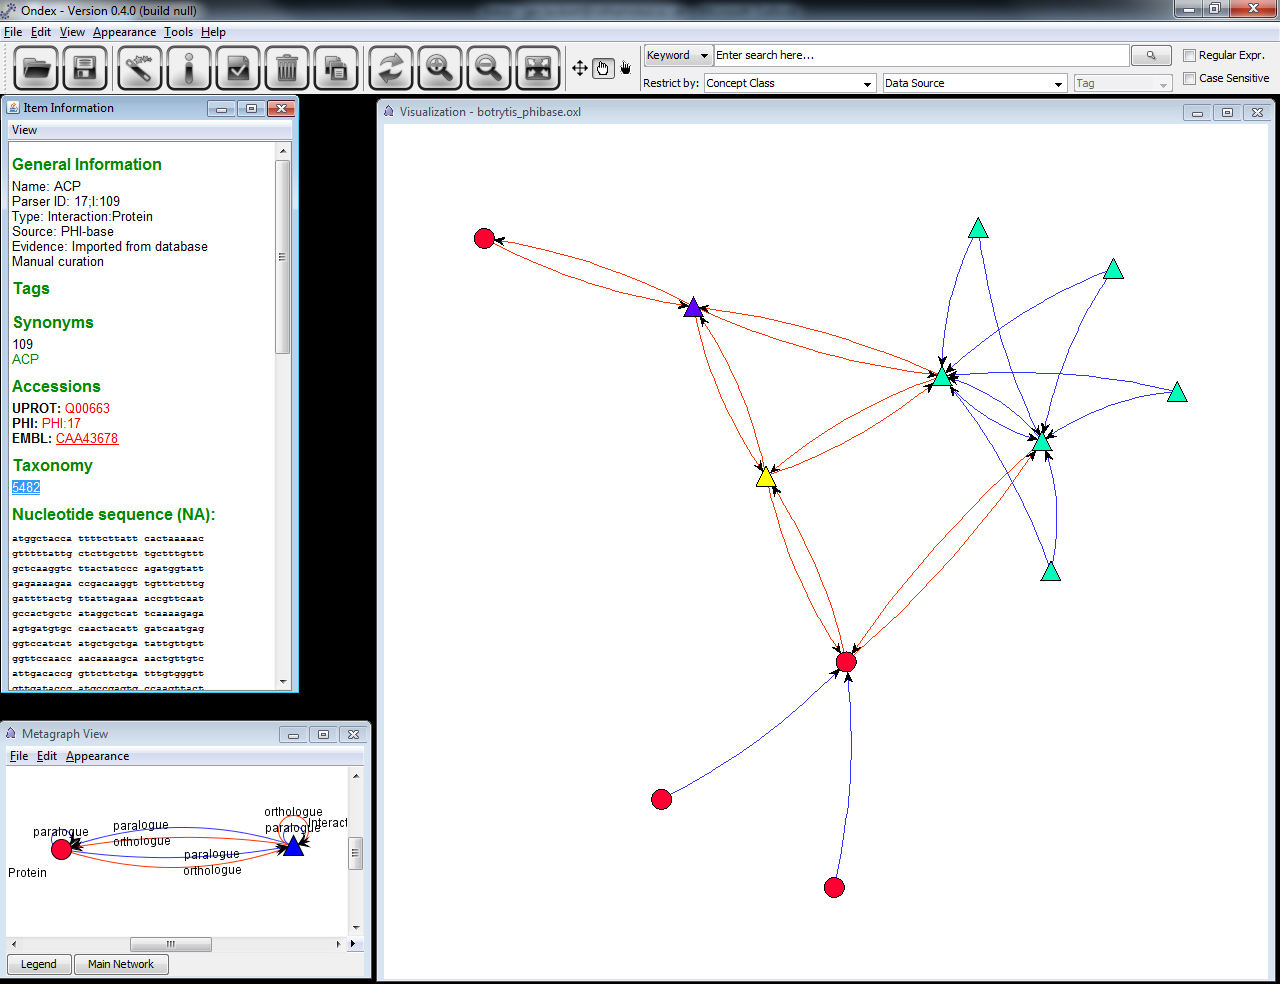
\includegraphics[scale=0.35]{images/Oct12/app2fig7.png} 
\caption{Taxonomy identifier in Item Information}
\label{fig:bot_taxid_lookup1}
\end{figure}

Once you know what Taxonomy identifier a concept holds, you may enter it in the box below and choose a shape you would like to associate to it (see Figure \ref{fig:bot_shape_before}).

\begin{figure}[H]
\centering
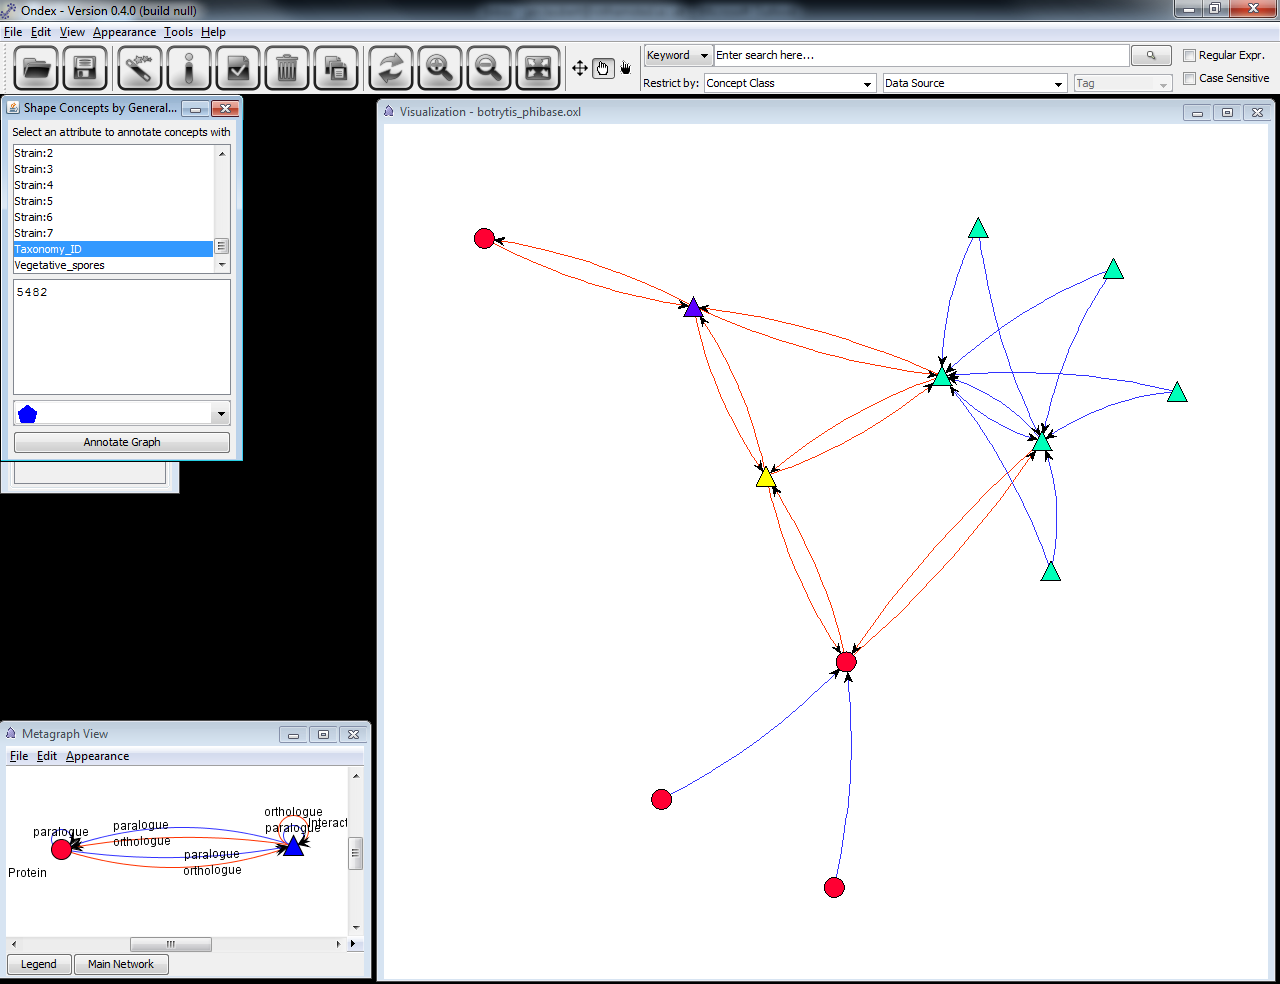
\includegraphics[scale=0.35]{images/Oct12/app2fig8.png} 
\caption{Applying the Shape Concepts by General Attribute annotator}
\label{fig:bot_shape_before}
\end{figure}

The results after clicking on ``Annotate Graph'' are shown on Figure \ref{fig:bot_shape_after}.

\begin{figure}[H]
\centering
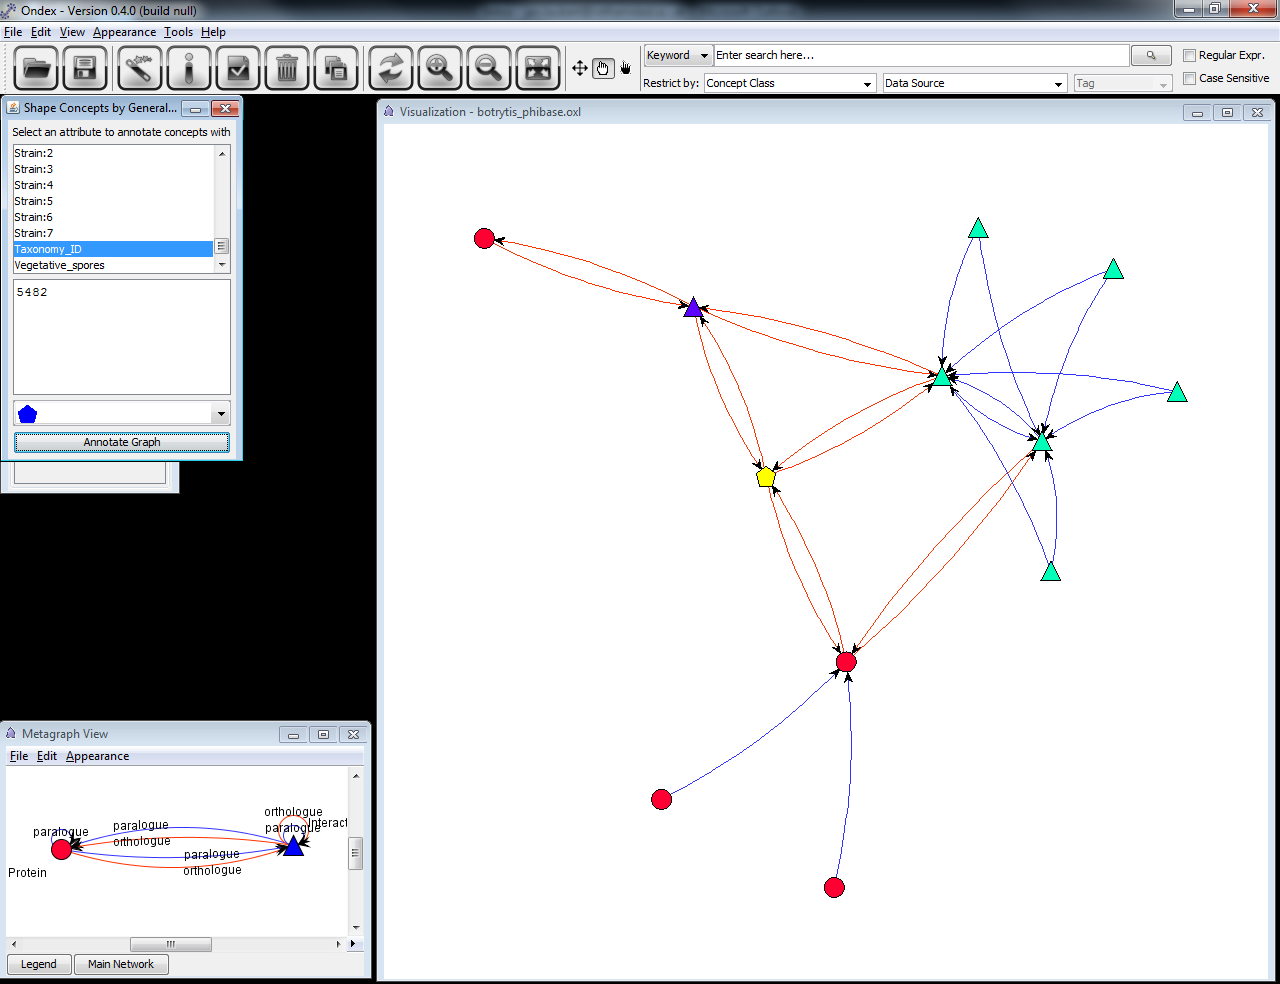
\includegraphics[scale=0.35]{images/Oct12/app2fig9.png} 
\caption{After applying the Shape Concepts by General Attribute annotator}
\label{fig:bot_shape_after}
\end{figure}

Let us change the shapes of all the PHI-base concepts in this cluster by using the same annotator several times (see Figures \ref{fig:bot_shape21} and \ref{fig:bot_shape22}). 
(Note: Entering more than one Taxonomy identifier in the blank box would make the same shape be associated to all of those Taxonomy identifiers.)

\begin{figure}[H]
\centering
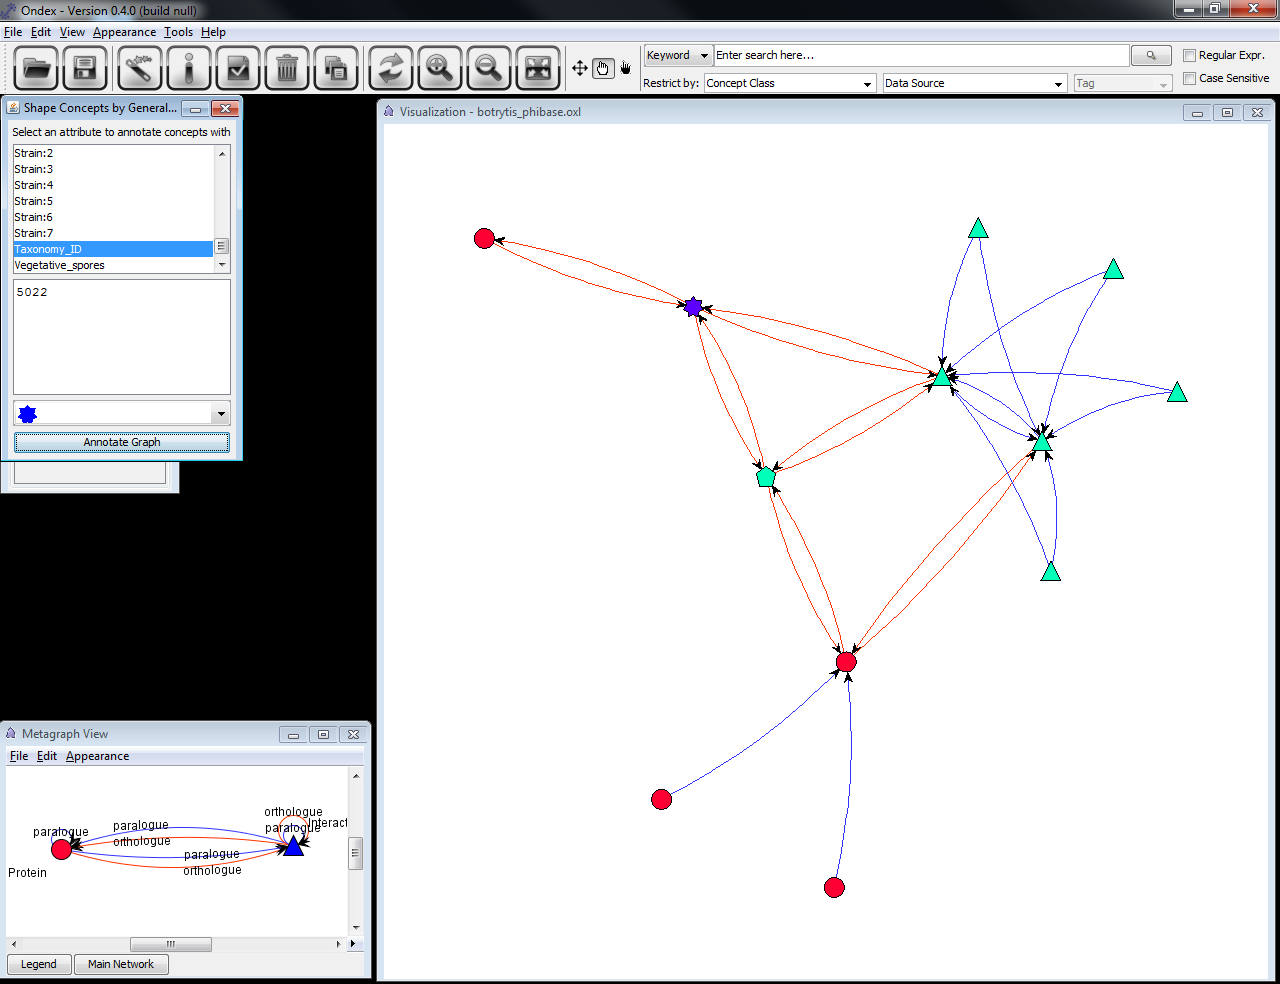
\includegraphics[scale=0.35]{images/Oct12/app2fig10.png} 
\caption{Applying the Shape Concepts by General Attribute annotator again}
\label{fig:bot_shape21}
\end{figure}

\begin{figure}[H]
\centering
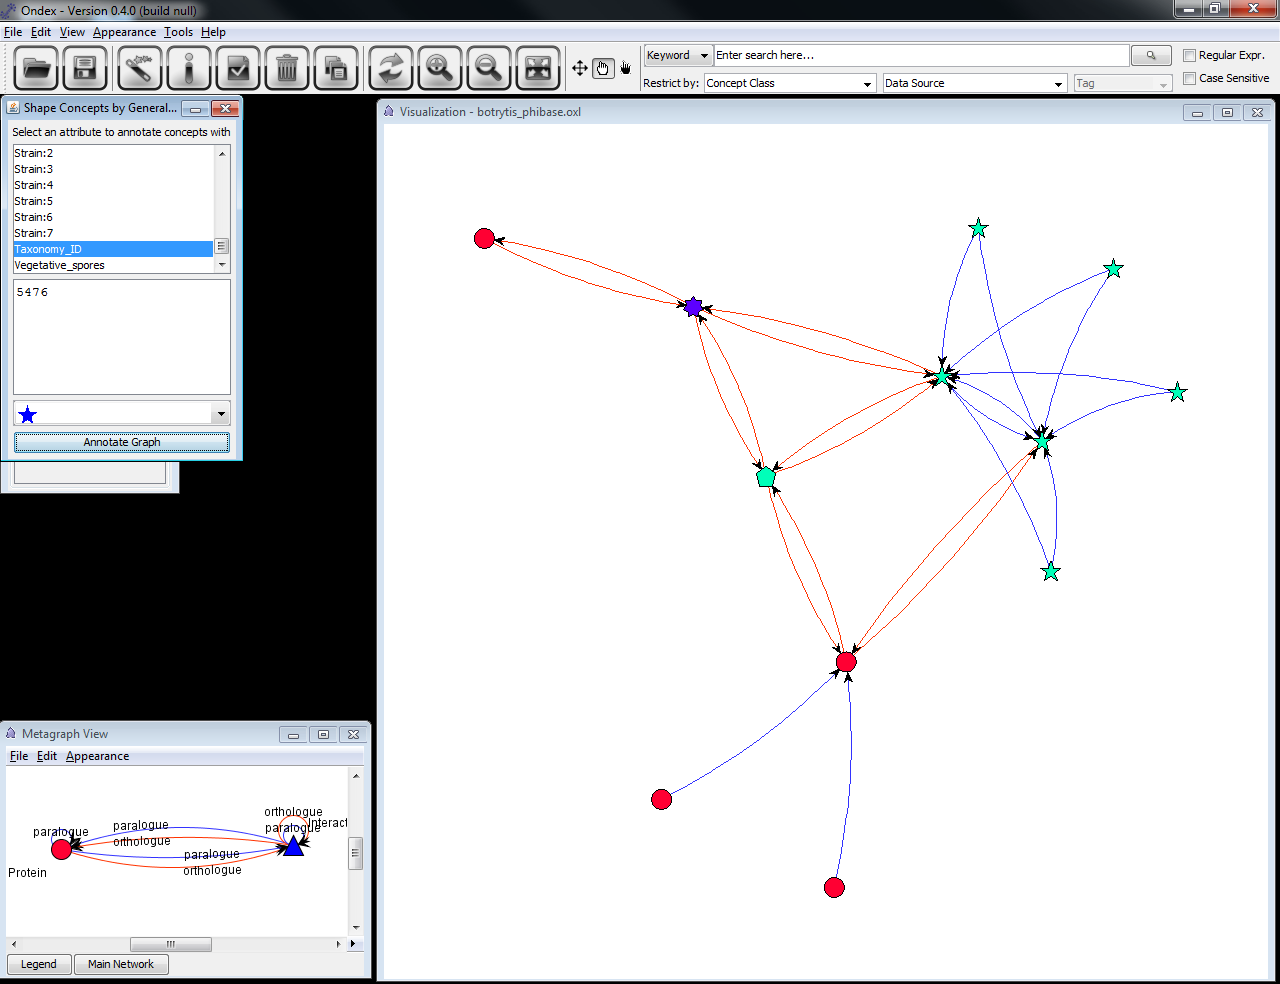
\includegraphics[scale=0.35]{images/Oct12/app2fig11.png} 
\caption{After applying the Shape Concepts by General Attribute annotator a third time}
\label{fig:bot_shape22}
\end{figure}
In this example we have shown how data integration combined with visualisation of annotations from a manually curated database 
can be used for guild-by-association studies to yield hypotheses for a newly sequenced genome.


\newpage
